\captionsetup{justification=centering}
\begin{figure}[H]
    \begin{subfigure}{1\textwidth}
        \centering
        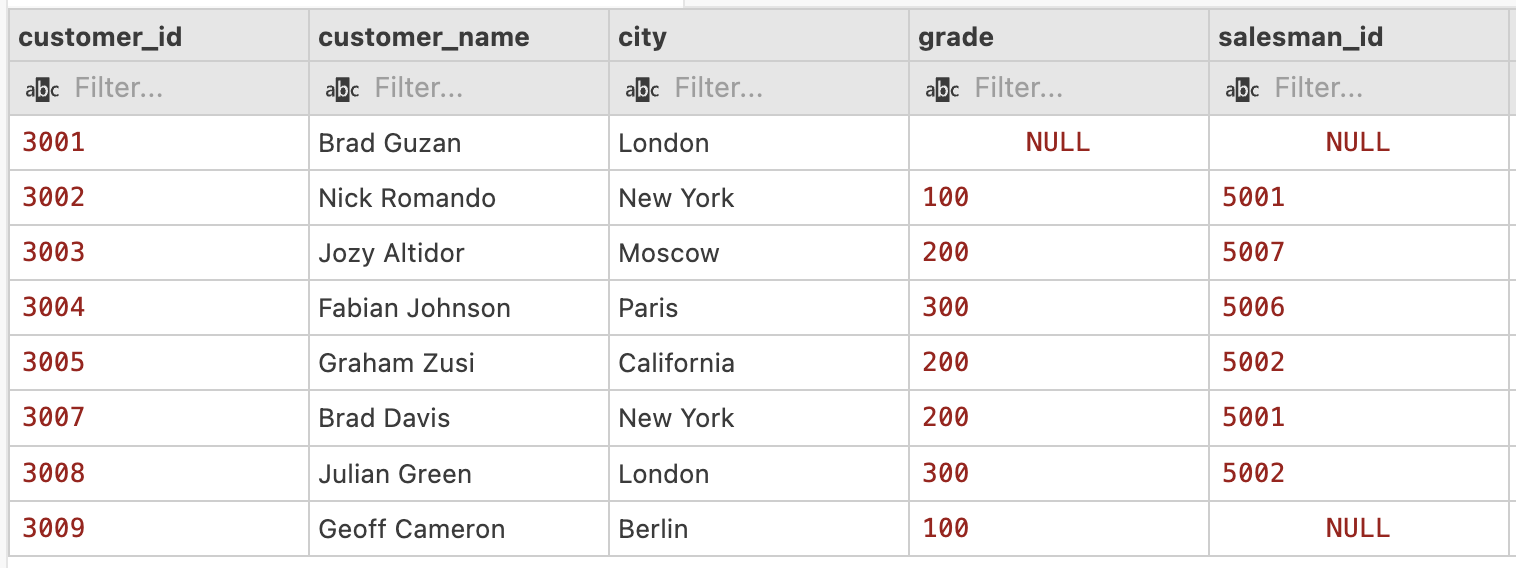
\includegraphics[width=.6\linewidth]{images/output/cust.png}
        \caption*{The complete Customer table.}
        \label{fig:cust}
    \end{subfigure}
    \begin{subfigure}{1\textwidth}
        \centering
        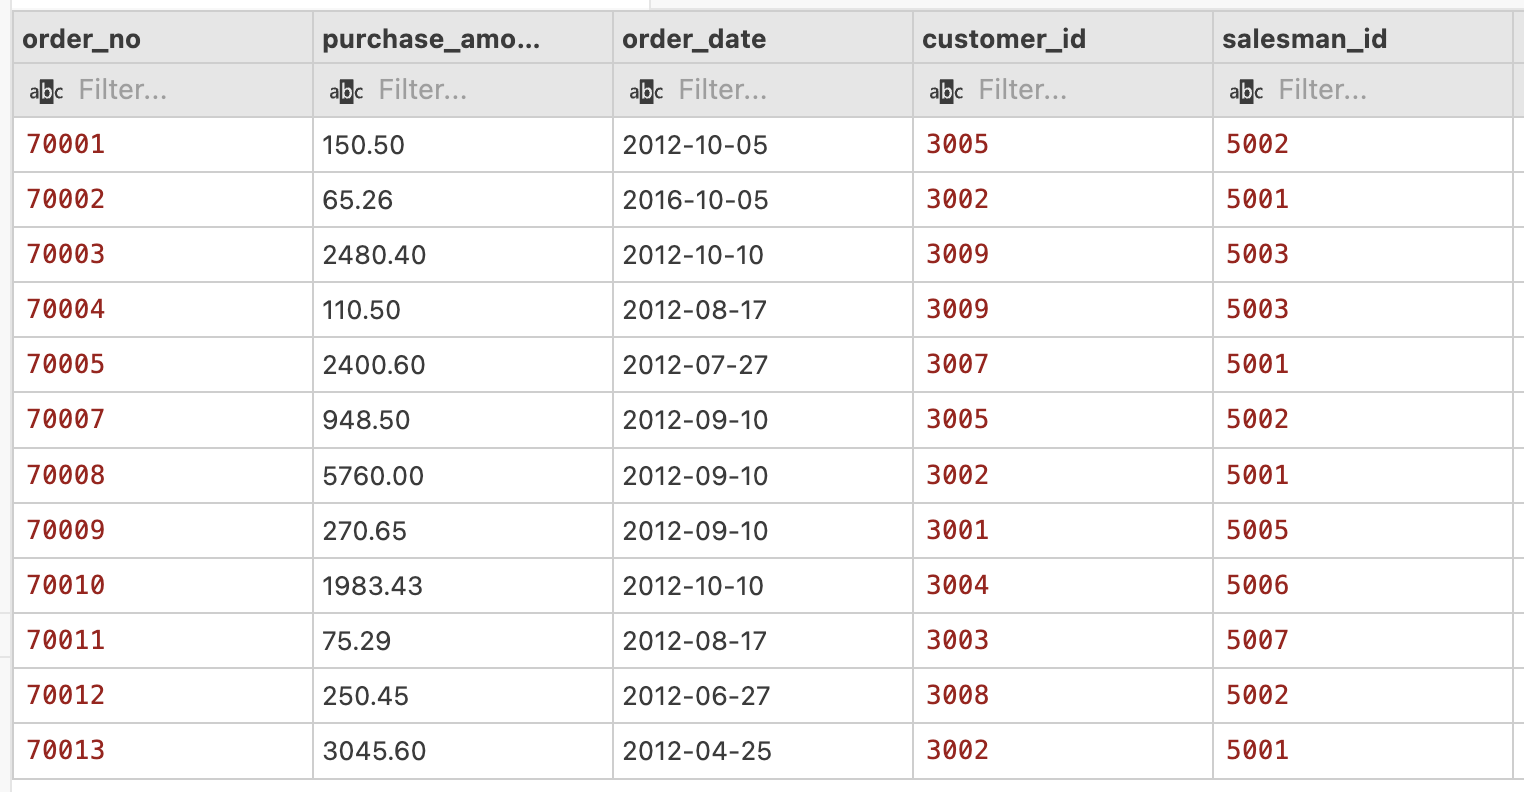
\includegraphics[width=.6\linewidth]{images/output/order.png}
        \caption*{The complete Order table.}
        \label{fig:ord}
    \end{subfigure}
    \vspace*{10mm}
    \begin{subfigure}{1\textwidth}
        \centering
        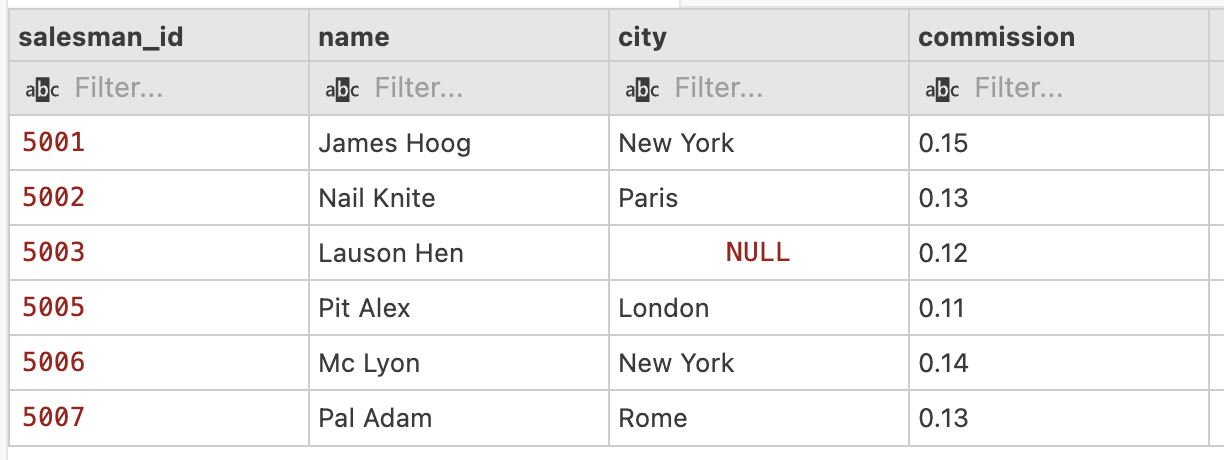
\includegraphics[width=.6\linewidth]{images/output/sman.png}
        \caption*{The complete Salesman table.}
        \label{fig:sman}
    \end{subfigure}
    \vspace*{10mm}
    \begin{subfigure}{.5\textwidth}
        \centering
        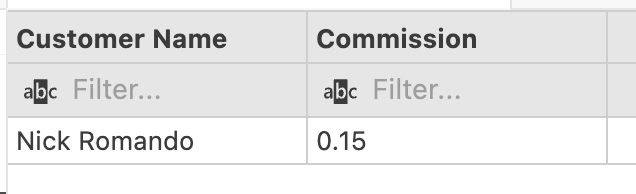
\includegraphics[width=.8\linewidth]{images/output/q1.png}
        \caption*{Customer who are given highest commission.}
        \label{fig:q1}
    \end{subfigure}
    \begin{subfigure}{.5\textwidth}
        \centering
        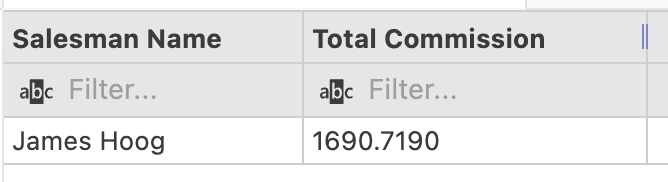
\includegraphics[width=.8\linewidth]{images/output/q2.png}
        \caption*{Amount of total commission given by salesman\_id = "5001"}
        \label{fig:q2}
    \end{subfigure}
    \begin{subfigure}{.5\textwidth}
        \centering
        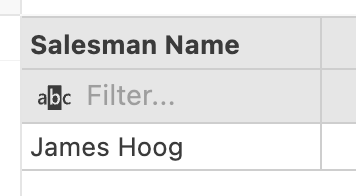
\includegraphics[width=.8\linewidth]{images/output/q3.png}
        \caption*{Salesman name whose customer’s grade is lowest.}
        \label{fig:q3}
    \end{subfigure}
    \begin{subfigure}{.5\textwidth}
        \centering
        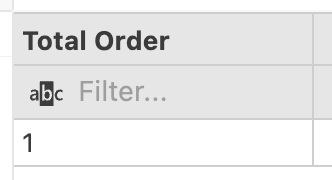
\includegraphics[width=.8\linewidth]{images/output/q4.png}
        \caption*{Total order number from 5-9-2016 to 17-10-2016}
        \label{fig:q4}
    \end{subfigure}
\end{figure}
